\chapter{Small wedges}
\label{ch:small}

In this chapter
we apply numerical boundary tracing to analyse corner rounding
in small capillary wedges,
for which the wedge half-angle~$\alpha$ and the contact angle~$\gamma$
satisfy the inequality~$\alpha < \pi/2 - \gamma$,
and for which the height rise in the corner is infinite.
After obtaining similar results to those in Chapter~\ref{ch:moderate}
for the rounding of moderate convex wedges,
we drop the insistence on smooth curves
and consider more general forms of corner modification,
by building on a comparison result
obtained by
Anderson~\cite[Section~7.3.2]{anderson-2002-thesis-boundary-tracing-pdes}.

\thematicbreak

The author's Honours thesis~%
  \cite{li-2017-thesis-rounding-capillary-wedge}
considered an asymptotic version of boundary tracing
in which the leading term~(\ref{eq:small-wedge-asymptotic-solution})
was used as the known solution.
Although that analysis was able to produce
a corresponding asymptotic rounding of the corner,
one could not be certain that this curve actually lay
within the region of validity
of the asymptotic known solution~(\ref{eq:small-wedge-asymptotic-solution}).
The accuracy of the asymptotic rounding curve
could only be assessed indirectly
by computing a numerical solution in the corresponding rounded-corner domain
(which no longer had a singularity)
and then comparing it
to the asymptotic solution~(\ref{eq:small-wedge-asymptotic-solution}).

It is more preferable to avoid the use of an asymptotic approximation,
so that the results of boundary tracing are applicable throughout the wedge,
rather than only in a near-corner region of unknown size.
Therefore, we determine here a numerical solution
to the scaled capillary BVP~(\ref{eq:scaled-laplace-young})
\&~(\ref{eq:scaled-contact-boundary-condition})
and apply boundary tracing to it,
instead of to an asymptotic solution.

\section{Numerical wedge solutions}
\label{sec:small.numerical}

While the numerical solver of Section~\ref{sec:moderate.nonlinear.numerical}
was able to generate solutions in the small wedge case,
the validity of these solutions is questionable
given the $1/r$~singularity in the corner.

A better approach involves extracting the singularity
before performing numerical work.
Such an approach has been employed by
Aoki \&~De~Sterck~\cite{aoki-2014-numerical-study-unbounded-capillary}
to determine accurate numerical representations
of unbounded solutions to the capillary problem,
specifically in the case of a general domain with two boundary walls,
$y = f (x)$ and $y = g (x)$,
forming either a small wedge or a cusp at the origin.
In this scenario,
the solution to the capillary problem~(\ref{eq:scaled-laplace-young})
\&~(\ref{eq:scaled-contact-boundary-condition})
is unbounded at the origin,
with the asymptotic height rise being of order~$1 / (f - g)$.
Their method consists of two parts.
The first is the change of dependent variable
\begin{equation}
  T (x, y) = \frac{H (x, y)}{f (x) - g(x)},
  \label{eq:capillary-unbounded-change-of-variable}
\end{equation}
which ensures that the new dependent variable~$H$ is bounded.
The second is the change of coordinates
\begin{align}
  x &= X,
    \label{eq:capillary-unbounded-x-transformation} \\
  y &= \frac{1 + Y}{2} f (X) + \frac{1 - Y}{2} g (X),
    \label{eq:capillary-unbounded-y-transformation}
\end{align}
which maps the original domain $x > 0$, $g (x) < y < f (x)$
to the rectangle $X > 0$, $-1 < Y < 1$.
In particular, this maps the origin~$(x, y) = (0, 0)$
to the line segment $X = 0$, $-1 < Y < 1$,
so that any discontinuity in~$H$ at the origin
(i.e.~a dependence on the direction of approach)
in the original coordinates~$(x, y)$
will not be exhibited in the new coordinates~$(X, Y)$.

The transformation~(\ref{eq:capillary-unbounded-x-transformation})
\&~(\ref{eq:capillary-unbounded-y-transformation})
is most general,
allowing the walls of the wedge or cusp to be curved.
Note that the new coordinates~$(X, Y)$ are not orthogonal.
In the present situation
we seek numerical solutions in wedge domains with straight walls,
namely domains of the form
$0 < r < 10$, $-\alpha < \phi < \alpha$
in polar coordinates.
Requiring not the generality of~(\ref{eq:capillary-unbounded-x-transformation})
\&~(\ref{eq:capillary-unbounded-y-transformation}),
but nevertheless inspired by the overall idea,
we implement here a similar transformation in polar coordinates
(which are orthogonal).

\subsection{Singularity extraction}
\label{sec:small.numerical.extraction}

After scaling out the capillary length~(\ref{eq:capillary-length})
as before,
the asymptotic height rise~(\ref{eq:small-wedge-asymptotic-solution})
in a small wedge reduces to
\begin{equation}
  T \asy \frac{\cos\phi - \sqrt{k^2 - \sin^2 \phi}}{k r},
  \label{eq:small-wedge-scaled-asymptotic-solution}
\end{equation}
where $k$~is given by~(\ref{eq:wedge-constant-k}), i.e.
\begin{equation}
  k = \frac{\sin\alpha}{\cos\gamma}.
  \label{eq:small-wedge-constant-k}
\end{equation}
In analogy to~(\ref{eq:capillary-unbounded-change-of-variable}),
we apply the transformation
\begin{equation}
  \savecontent{
    T (r, \phi) = \frac{H (r, \phi)}{r}
  }{eq:small-wedge-change-of-variable}
\end{equation}
so that the new dependent variable~$H$ is bounded and continuous
(in the sense of single-valuedness for~$-\alpha < \phi < \alpha$)
at~$r = 0$.

Now the numerical BVP solver of \software{Mathematica}
can only handle rectangular coordinates.
Coefficient matrices are always interpreted
as components of a rectangular coordinate system,
and if the list of independent variables supplied is~$(u, v)$,
the corresponding list of derivative operators
will be~$(\pd / {\pd u}, \pd / {\pd v})$,
which does not accord with
the physical gradient and divergence operators
unless the scale factors are unity.
Indeed the polar coordinate system is not rectangular,
so we must first rewrite the capillary problem~(\ref{eq:scaled-laplace-young})
\&~(\ref{eq:scaled-contact-boundary-condition})
in terms of~$(\pd / {\pd r}, \pd / {\pd\phi})$,
so that $r$ and~$\phi$ may be interpreted formally
as rectangular coordinates.

After effecting the transformation~(\ref{eq:small-wedge-change-of-variable})
(see Appendix~\ref{ch:extraction}\@),
the capillary problem~(\ref{eq:scaled-laplace-young})
\&~(\ref{eq:scaled-contact-boundary-condition}) in~$T$
becomes the BVP
\begin{align}
  \matder \dotp \squarebr[\bulkysize]{\mat{K} \matder H - \mat{v} H}
    &= H,
    \label{eq:small-formally-rectangular-laplace-young} \\
  \mat{n} \dotp \squarebr[\bulkysize]{\mat{K} \matder H - \mat{v} H}
    &= \cos\gamma
    \label{eq:small-formally-rectangular-contact-boundary-condition}
\end{align}
in~$H$, where
\begin{align}
  \matder &=
    \begin{pmatrix}
      \pd / {\pd r} \\
      \pd / {\pd\phi}
    \end{pmatrix},
    \label{eq:small-formally-rectangular-derivative} \\
  \saveequation{
    \mat{K}
  }{&=}{
    \begin{pmatrix}
      r^2 C & 0 \\
      0 & C
    \end{pmatrix}
  }{eq:small-formally-rectangular-diffusion-coefficient}, \\
  \saveequation{
    \mat{v}
  }{&=}{
    \begin{pmatrix}
      r C \\
      0
    \end{pmatrix}
  }{eq:small-formally-rectangular-convection-coefficient},
\end{align}
and $\mat{n}$~is to~$\matder$ as $\normalvec$~is to~$\del$,
with
\begin{equation}
  \savecontent{
    C = \frac{1}{\sqrt{r^4 + \desing{P}^2 + \desing{Q}^2}}
  }{eq:small-formally-rectangular-scalar-coefficient},
\end{equation}
where
\begin{align}
  \desing{P} &= r \pder{H}{r} - H,
    \label{eq:small-gradient-de-singularised-r-component}
    \\[\tallspace]
  \desing{Q} &= \pder{H}{\phi}.
    \label{eq:small-gradient-de-singularised-phi-component}
\end{align}
The transformed problem~(\ref{eq:small-formally-rectangular-laplace-young})
\&~(\ref{eq:small-formally-rectangular-contact-boundary-condition})
is to be solved in the region
$0 < r < 10$, $-\alpha < \phi < \alpha$,
which algebraically has the form of a rectangle
(Figure~\ref{fig:wedge_small-domain-formal-rectangle}).
Note that $\mat{n}$~is not a physical normal vector,
and that $\matder$~is not a physical vector operator.
Only $\normalvec$ and~$\del$ have a physically meaningful interpretation
in association with the original wedge
(Figure~\ref{fig:wedge_small-domain-original-wedge}).
While it is useful to think of~$\mat{n}$ and~$\matder$
as analogous entities for the rectangle of
Figure~\ref{fig:wedge_small-domain-formal-rectangle},
they are merely algebraic tools for computing~$H$
using a numerical solver that assumes a rectangular coordinate system.

\begin{figure}
  \newcommand*{\subfigurewidth}{0.3\textwidth}
  \centering
  \hspace*{\fill}
  \begin{subfigure}[t]{\subfigurewidth}
    \centredfigurecontent{wedge_small-domain-original-wedge}{%
      Original wedge
    }
  \end{subfigure}
    \hfill
  \begin{minipage}[t]{0.25\textwidth}
    \centering
    \includegraphics[width=\textwidth, trim=0 {-0.35\textwidth} 0 0]{%
      wedge_small-domain-double-arrow%
    }
  \end{minipage}
    \hfill
  \begin{subfigure}[t]{\subfigurewidth}
    \centredfigurecontent{wedge_small-domain-formal-rectangle}{%
      Formal rectangle
    }
  \end{subfigure}
  \hspace*{\fill}
  \caption{
    Alternative interpretations of the domain
    $0 < r < 10$, $-\alpha < \phi < \alpha$.
  }
  \label{fig:wedge_small-domain}
\end{figure}

\subsection{Implementation}
\label{sec:small.numerical.implementation}

The rectangle of Figure~\ref{fig:wedge_small-domain-formal-rectangle}
is discretised into an unstructured triangular mesh.
The minimalistic refinement strategy
of Section~\ref{sec:moderate.nonlinear.numerical.half-plane}
is applied
along~$r = 0$ (which represents the wedge corner)
and~$\phi = \pm\alpha$ (which represent the wedge walls)
using a fine length scale of~$0.01$.
To ensure that first derivatives
can also be computed accurately elsewhere
for the purposes of boundary tracing,
a coarser uniform refinement is also applied throughout the mesh,
such that no mesh element has more area than the equilateral triangle
whose side length is the lesser of~$0.1$ and~$\alpha / 5$.
An example mesh is shown in
Figure~\ref{fig:wedge_small-mesh-detail}.

\begin{figure}
  \centredfigurecontent[width=0.8\textwidth]{%
    wedge_small-mesh-detail%
  }{
    Portion of the finite element mesh
    for an $\alpha = \SI{30}{\degree}$~formal rectangle.
  }
\end{figure}

While the PDE~(\ref{eq:small-formally-rectangular-laplace-young})
is applied throughout the rectangular region,
the boundary condition~%
  (\ref{eq:small-formally-rectangular-contact-boundary-condition})
as written
is only used along the boundaries~$\phi = \pm\alpha$
representing the wedge walls.
Along the boundary~$r = 10$ we instead use the non-wetting version
\begin{equation}
  \mat{n} \dotp \squarebr[\bulkysize]{\mat{K} \matder H - \mat{v} H} = 0
  \label{eq:small-formally-rectangular-natural-boundary-condition}
\end{equation}
(equivalent to setting~$\gamma = \pi/2$)
to model a vanishing height rise at infinity.
It remains to specify the boundary condition along the boundary~$r = 0$,
which represents the corner of the original wedge.
Defining the angular function
\begin{equation}
  H_0 = \frac{\cos\phi - \sqrt{k^2 - \sin^2 \phi}}{k},
  \label{eq:small-asymptotic-angular-function}
\end{equation}
the asymptotic relation~(\ref{eq:small-wedge-scaled-asymptotic-solution})
for small~$r$ becomes
\begin{equation}
  T \asy \frac{H_0}{r},
  \label{eq:small-asymptotic-solution}
\end{equation}
and we see that a suitable boundary condition to apply along~$r = 0$
is the Dirichlet condition
\begin{equation}
  H = H_0.
  \label{eq:small-formally-rectangular-dirichlet-condition}
\end{equation}

Although \software{Mathematica~12}'s built-in numerical solver
can handle nonlinear problems using Newton's method,
convergence issues arise for the BVP at hand.
We therefore implement a custom fixed-point iteration instead,
at each step supplying a linearised BVP
by pre-evaluating the coefficients~$\mat{K}$ and~$\mat{v}$
using the solution computed from the previous step.
For the initial guess we use
the asymptotic angular function~(\ref{eq:small-asymptotic-angular-function}).
While fixed-point iteration is slower than Newton's method,
it is very robust, and we do not encounter any problems with convergence.
Selected results are shown in Figure~\ref{fig:wedge_small-solution}.

\begin{figure}
  \newcommand*{\subfigurewidth}{0.45\textwidth}
  \centering
  \begin{subfigure}[t]{\subfigurewidth}
    \centredfigurecontent{%
      wedge_small-solution-small%
    }{%
      $\gamma = \SI{45}{\degree}$ (small regime)
    }
  \end{subfigure}
    \hfill
  \begin{subfigure}[t]{\subfigurewidth}
    \centredfigurecontent{%
      wedge_small-solution-borderline%
    }{%
      $\gamma = \SI{60}{\degree}$ (borderline case)
    }
  \end{subfigure}
  \caption{
    Radial profiles (for both~$H$ and~$T$) of selected numerical solutions
    in an $\alpha = \SI{30}{\degree}$~wedge.
    Curves from bottom to top:
    $\phi =
      \SI{0}{\degree}, \SI{10}{\degree},
      \SI{20}{\degree}, \SI{30}{\degree}$.
  }
  \label{fig:wedge_small-solution}
\end{figure}

It is interesting to note that
the numerical scheme is able to produce a sensible result
even in the borderline case~$\alpha = \pi/2 - \gamma$,
where the height rise in the corner is finite.
While the transformation~(\ref{eq:small-wedge-change-of-variable})
appears at first glance to preclude a bounded solution in~$T$,
the borderline case has~$k = 1$,
and hence an identically-vanishing
asymptotic angular function~(\ref{eq:small-asymptotic-angular-function}).
The Dirichlet condition~%
  (\ref{eq:small-formally-rectangular-dirichlet-condition})
therefore reduces to~$H = 0$,
and the singularity at~$r = 0$ is eliminated.
While it is possible to estimate the height rise~$T$ in the corner
by extrapolating the computed value of~$H / r$ to~$r = 0$,
we should not expect a high level of accuracy
due to (multiplicative) catastrophic cancellation
between~$H$ (going to zero) and~$1 / r$ (going to infinity).
We may compare $T = H / r$~obtained here using
the polar-coordinate transformation~(\ref{eq:small-wedge-change-of-variable})
with the corresponding numerical solution
obtained in Section~\ref{sec:moderate.nonlinear.numerical.wedge}
by directly using the Cartesian-based BVP solver.
Figure~\ref{fig:wedge_small-borderline-comparison}
shows the relative discrepancy
\begin{equation}
  \abs*{\frac{\textq{Polar~$T$}}{\textq{Cartesian~$T$}} - 1}
  \label{eq:wedge_small-relative-discrepancy-with-cartesian}
\end{equation}
between the two approaches
for the specific example of~$\alpha = \SI{30}{\degree}$.
As expected,
the discrepancy of~$\SI{10}{\percent}$ at~$r = 0$
is not exceedingly small,
but as we move away from the corner,
the discrepancy decreases very quickly.
The fact that two very different approaches
produce numerical solutions in close agreement
allows us to be confident in the results of both.

\begin{figure}
  \centredfigurecontent[width=!, height=0.35\textwidth]{%
    wedge_small-borderline-comparison%
  }{
    Relative discrepancy~%
      (\ref{eq:wedge_small-relative-discrepancy-with-cartesian})
    between polar- and Cartesian-based numerical solutions,
    for the borderline case~%
    $(\alpha, \gamma) = (\SI{30}{\degree}, \SI{60}{\degree})$.
  }
\end{figure}

\section{Corner rounding}
\label{sec:small.rounding}

Having obtained numerical solutions~$T = H / r$ for small wedges,
we now use boundary tracing to seek rounding shapes
which still satisfy the contact condition~%
  (\ref{eq:scaled-contact-boundary-condition}).
Again after writing this in the standard form
\begin{important}{equation}
  \normalvec \dotp \del T = \cos\gamma \sqrt{1 + (\del T)^2},
  \label{eq:small-flux-boundary-condition}
\end{important}
we see that the flux function is
\begin{equation}
  F = \cos\gamma \sqrt{1 + (\del T)^2}.
  \label{eq:small-flux-function}
\end{equation}

\subsection{Wedge solution derivatives}
\label{sec:small.rounding.derivatives}

To perform boundary tracing,
we need to evaluate first derivatives of the wedge solution~$T$.
Since it is~$H$ (not~$T$) that we have computed,
we begin by expressing the relevant derivatives of~$T$
in terms of derivatives of~$H$.

First we observe that the components of~$\del T$ are of order~$1 / r^2$.
Indeed we have
\begin{align}
  P &= \pder{T}{r}
    = \frac{1}{r} \pder{H}{r} - \frac{H}{r^2}
    = \frac{\desing{P}}{r^2},
      \label{eq:small-gradient-r-component} \\[\tallspace]
  Q &= \frac{\pd T}{r \pd\phi}
    = \frac{1}{r^2} \pder{H}{\phi}
    = \frac{\desing{Q}}{r^2},
      \label{eq:small-gradient-phi-component}
\end{align}
where the de-singularised versions~$\desing{P}$ and~$\desing{Q}$
are defined by~(\ref{eq:small-gradient-de-singularised-r-component})
and~(\ref{eq:small-gradient-de-singularised-phi-component})
in terms of derivatives of~$H$.
Therefore
\begin{equation}
  (\del T)^2
    = P^2 + Q^2
    = \frac{\desing{P}^2 + \desing{Q}^2}{r^4},
  \label{eq:small-gradient-squared}
\end{equation}
and the flux function~(\ref{eq:small-flux-function}) becomes
\begin{equation}
  F
    =
      \cos\gamma
      \sqrt{1 + \frac{\desing{P}^2 + \desing{Q}^2}{r^4}}
    =
      \frac{\desing{F}}{r^2},
    \label{eq:small-flux-function-singular}
\end{equation}
where
\begin{equation}
  \desing{F} = \cos\gamma \sqrt{r^4 + \desing{P}^2 + \desing{Q}^2}.
  \label{eq:small-flux-function-de-singularised}
\end{equation}
Likewise for the viability function~$\Phi$,
given again by~(\ref{eq:moderate-viability-function}),
we have
\begin{equation}
  \Phi
    =
      \sin^2\gamma \cdot \frac{\desing{P}^2 + \desing{Q}^2}{r^4}
      - \cos^2\gamma
    =
      \frac{\desing{\Phi}}{r^4},
    \label{eq:small-viability-function-singular}
\end{equation}
where
\begin{equation}
  \desing{\Phi} =
    \sin^2\gamma \, \roundbr*{\desing{P}^2 + \desing{Q}^2} - r^4 \cos^2\gamma
  \label{eq:small-viability-function-de-singularised}
\end{equation}
is the de-singularised version.
Since $\Phi$ and~$\desing{\Phi}$ have the same sign everywhere,
the viable domain is the region
\begin{equation}
  \desing{\Phi} \ge 0.
  \label{eq:small-viable-domain}
\end{equation}
As in the moderate convex wedge case,
the viable domain lies to the left
and the non-viable domain lies to the right
(Figure~\ref{fig:wedge_small-viable}).
The terminal curve
\begin{equation}
  \desing{\Phi} = 0
  \label{eq:small-terminal-curve}
\end{equation}
demarcates the two regions,
and approaches the walls of the wedge
as one travels away from the line of symmetry~$y = 0$.

\begin{figure}
  \newcommand*{\legendoffsetheight}{0.255\textwidth}
  \centering
  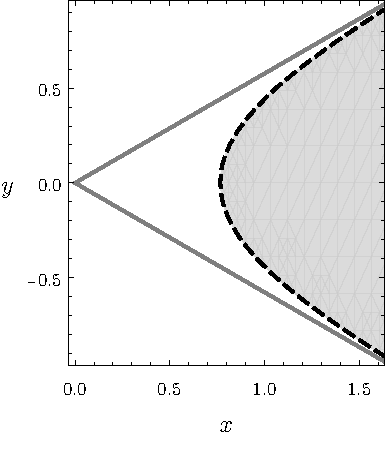
\includegraphics[width=0.45\textwidth]{wedge_small-viable}
  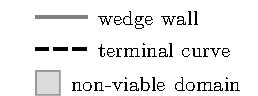
\includegraphics[
    width=0.3\textwidth,
    trim=0 {-\legendoffsetheight} 0 0,
  ]{wedge_small-viable-legend}
  \caption{
    Non-viable domain~$\desing{\Phi} < 0$
    for~$\alpha = \SI{30}{\degree}$ and~$\gamma = \SI{45}{\degree}$.
  }
  \label{fig:wedge_small-viable}
\end{figure}

\subsection{Boundary tracing}
\label{sec:small.rounding.tracing}

We now proceed to actually performing boundary tracing.
Working in polar coordinates~$(r, \phi)$,
the boundary tracing system of ODEs~%
  (\ref{eq:tracing-ode-arc-length-parametrisation-u})
\&~%
  (\ref{eq:tracing-ode-arc-length-parametrisation-v})
for arc-length parametrisation
becomes
\begin{align*}
  \tder{r}{s} &= \frac{-Q F \pm P \sqrt{\Phi}}{P^2 + Q^2},
    \\[\tallspace]
  \tder{\phi}{s} &= \frac{+P F \pm Q \sqrt{\Phi}}{r \roundbr*{P^2 + Q^2}}.
\end{align*}
Now the numerators and denominators in both equations
are all quadratic in~$P$, $Q$, $F$, and~$\sqrt{\Phi}$,
which quantities are all equal to $1 / r^2$~multiplied by
their de-singularised equivalents (with \desingmarks).
We may therefore simply insert \desingmarks{} to obtain
\begin{important}{align}
  \tder{r}{s} &=
    \frac{
      -\desing{Q} \desing{F} \pm \desing{P} \sqrt{\desing{\Phi}}
    }{
      \desing{P}^2 + \desing{Q}^2
    },
    \label{eq:small-tracing-ode-arc-length-parametrisation-r}
    \\[\tallspace]
  \tder{\phi}{s} &=
    \frac{
      +\desing{P} \desing{F} \pm \desing{Q} \sqrt{\desing{\Phi}}
    }{
      r \roundbr*{\desing{P}^2 + \desing{Q}^2}
    },
    \label{eq:small-tracing-ode-arc-length-parametrisation-phi}
\end{important}
whose right-hand sides may be readily evaluated
according to the de-singularised expressions determined in
Section~\ref{sec:small.rounding.derivatives}.

\begin{figure}
  \newcommand*{\legendoffsetheight}{0.25\textwidth}
  \centering
  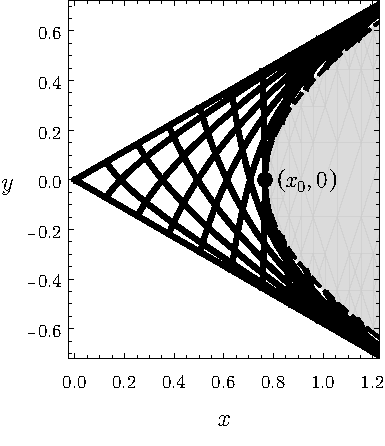
\includegraphics[width=0.45\textwidth]{wedge_small-traced-boundaries}
  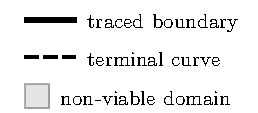
\includegraphics[
    width=0.3\textwidth,
    trim=0 {-\legendoffsetheight} 0 0,
  ]{wedge_acute-traced-boundaries-legend}
  \caption{
    Traced boundaries for~$\alpha = \SI{30}{\degree}$
    and~$\gamma = \SI{45}{\degree}$,
    obtained by integrating~%
      (\ref{eq:small-tracing-ode-arc-length-parametrisation-r})
    \&~%
      (\ref{eq:small-tracing-ode-arc-length-parametrisation-phi}).
  }
  \label{fig:wedge_small-traced-boundaries}
\end{figure}

By performing numerical integration
from various starting points in the viable domain,
we obtain the traced boundaries shown
in Figure~\ref{fig:wedge_small-traced-boundaries}.
As before, these traced boundaries may be patched together
to form an unlimited number of new domain boundaries
like those in Figure~\ref{fig:wedge_acute-traced-boundaries-patched},
but sharp corners will be formed
\emph{strictly} within the viable domain.
Thus, we again look to the terminal curve
in our search for a rounding of the wedge.
The manner in which the $T$-contours cross the terminal curve
is qualitatively identical to Figure~\ref{fig:wedge_acute-terminal-points}
(for the moderate wedge case).
Almost all terminal points are ordinary (and hence not useful),
with the sole exception being
the hyperbolic critical terminal point~$(x, y) = (x_0, 0)$
which lies at the intersection between
the terminal curve~(\ref{eq:small-terminal-curve})
and the line of symmetry~$y = 0$.
Algebraically, $r = x_0$~is the unique solution to the equation
\begin{equation}
  \eval*{-\frac{\desing{P}}{r^2}}_{\phi=0} = \cot\gamma.
  \label{eq:small-critical-terminal-point}
\end{equation}
Two smooth traced boundaries pass through
the critical terminal point~$(x_0, 0)$,
with the portions to the right forming a rounding of the corner
(Figure~\ref{fig:wedge_small-traced-boundaries-hyperbolic}).
In Section~\ref{sec:moderate.nonlinear.approach}
we obtained the estimate~(\ref{eq:moderate-perturbation-near-wall-approach}),
for the rate at which the rounding curve approached the wedge walls
in a moderate convex wedge;
that result carries through without change
to the small wedge case here.

\begin{figure}
  \newcommand*{\subfigurewidth}{0.45\textwidth}
  \newcommand*{\subfiguregraphicswidth}{0.75\textwidth}
  \centering
  \hspace*{\fill}
  \begin{subfigure}[t]{\subfigurewidth}
    \centredfigurecontent[width=\subfiguregraphicswidth]{%
      wedge_small-traced-boundaries-hyperbolic-both%
    }{%
      Two smooth boundaries
    }
  \end{subfigure}
    \hfill
  \begin{subfigure}[t]{\subfigurewidth}
    \centredfigurecontent[width=\subfiguregraphicswidth]{%
      wedge_small-traced-boundaries-hyperbolic-rounding%
    }{%
      Rounding of the wedge corner
    }
  \end{subfigure}
  \hspace*{\fill}
  \caption{
    Traced boundaries through the critical terminal point~$(x_0, 0)$.
  }
  \label{fig:wedge_small-traced-boundaries-hyperbolic}
\end{figure}

\subsection{Different contact angle}
\label{sec:small.rounding.different}

Proceeding as in the moderate wedge case
(Section~\ref{sec:moderate.multiple.different}),
a single numerical wedge solution~$T (r, \phi; \alpha, \gamma)$
can be used to generate multiple roundings of the corner
for the boundary condition
\begin{important}{equation}
  \normalvec \dotp \del T (r, \phi; \alpha, \gamma) =
    \cos\gamma_\tr
    \sqrt{1 + \squarebr[\bulkysize]{\del T (r, \phi; \alpha, \gamma)}^2}
  \label{eq:small-flux-boundary-condition-different-angle}
\end{important}
corresponding to a different contact angle~$\gamma_\tr$.
With the de-singularised flux and viability functions
(\ref{eq:small-flux-function-de-singularised})
and~(\ref{eq:small-viability-function-de-singularised})
modified to become
\begin{equation}
  \desing{F} =
    \cos\gamma_\tr
    \sqrt{
      r^4
      + \desing{P}^2 (r, \phi; \alpha, \gamma)
      + \desing{Q}^2 (r, \phi; \alpha, \gamma)
    }
  \label{eq:small-flux-function-de-singularised-different-angle}
\end{equation}
and
\begin{equation}
  \desing{\Phi} =
    \sin^2\gamma_\tr \,
    \roundbr*{
      \desing{P}^2 (r, \phi; \alpha, \gamma)
        +
      \desing{Q}^2 (r, \phi; \alpha, \gamma)
    }
      - r^4 \cos^2\gamma_\tr,
  \label{eq:small-viability-function-de-singularised-different-angle}
\end{equation}
the boundary tracing system of ODEs~%
  (\ref{eq:small-tracing-ode-arc-length-parametrisation-r})
\&~%
  (\ref{eq:small-tracing-ode-arc-length-parametrisation-phi})
remains unchanged in form.
Integrating to obtain traced boundaries
(Figure~\ref{fig:wedge_small-traced-boundaries-different-angle}),
we again find that the viable domain does not extend to infinity
in the case of~$\gamma_\tr < \gamma$,
so that a rounding of the corner cannot be produced.

\begin{figure}
  \newcommand*{\subfigurewidth}{0.4\textwidth}
  \centering
  \includegraphics[width=\textwidth, trim=0 -7 0 0]{%
    wedge_acute-traced-boundaries-different-angle-legend%
  }
  \hspace*{\fill}
  \begin{subfigure}[t]{\subfigurewidth}
    \centredfigurecontent{%
      wedge_small-traced-boundaries-different-angle-less%
    }{%
      $\gamma_\tr = \SI{40}{\degree} < \gamma$
    }
  \end{subfigure}
    \hfill
  \begin{subfigure}[t]{\subfigurewidth}
    \centredfigurecontent{%
      wedge_small-traced-boundaries-different-angle-more%
    }{%
      $\gamma_\tr = \SI{55}{\degree} > \gamma$
    }
  \end{subfigure}
  \hspace*{\fill}
  \caption{
    Traced boundaries for~$\alpha = \SI{30}{\degree}$,
    $\gamma = \SI{45}{\degree}$, and~$\gamma_\tr \ne \gamma$,
    obtained by integrating~%
      (\ref{eq:small-tracing-ode-arc-length-parametrisation-r})
    \&~%
      (\ref{eq:small-tracing-ode-arc-length-parametrisation-phi}).
  }
  \label{fig:wedge_small-traced-boundaries-different-angle}
\end{figure}

For~$\gamma_\tr > \gamma$ the viable domain does extend to infinity,
and a candidate boundary can be constructed as before
by patching together traced boundaries through
the sole critical terminal point~$(x_0, 0)$,
where now $r = x_0$ is the unique solution to
\begin{equation}
  \eval*{
    -\frac{\desing{P}(r, \phi; \alpha, \gamma)}{r^2}
  }_{\phi=0}
    = \cot\gamma_\tr
  \label{eq:small-critical-terminal-point-different-angle}
\end{equation}
instead of~(\ref{eq:small-critical-terminal-point}).
The candidate boundary approaches a wedge offset from the original
by the perpendicular distance~$d (\gamma, \gamma_\tr)$
(Figure~\ref{fig:wedge_small-different-angle-offset-top}),
as it did in the moderate wedge case
(recall equation~(\ref{eq:moderate-offset-distance})
and Figure~\ref{fig:wedge_acute-different-angle-offset-side}).

\begin{figure}
  \centredfigurecontent[width=0.5\textwidth]{%
    wedge_small-different-angle-offset-top%
  }{%
    Top view of the candidate boundary approaching an offset wedge
    for~$\gamma_\tr > \gamma$.
  }
\end{figure}

\begin{figure}
  \centredfigurecontent[width=0.45\textwidth]{%
    wedge_small-candidates%
  }{%
    One-parameter family of candidate boundaries for~$\gamma_\tr \ge \gamma$,
    all obtained from the wedge solution
    for~$\alpha = \SI{30}{\degree}$ and~$\gamma = \SI{45}{\degree}$.
    From left to right:
    $\gamma_\tr =
      \SI{45}{\degree}, \SI{50}{\degree}, \dots, \SI{75}{\degree}$.
  }
\end{figure}

Thus, given a single numerical wedge solution~%
  $T (r, \phi; \alpha, \gamma) = H (r, \phi; \alpha, \gamma) / r$,
boundary tracing can be used to construct
a one-parameter family~$\gamma_\tr \ge \gamma$
of candidate boundaries for corner rounding;
an example is shown in Figure~\ref{fig:wedge_small-candidates}.
Although the procedure up to this point
has been no different to the moderate wedge case
(Section~\ref{sec:moderate.multiple.different}),
there is an interesting point of difference
in the present small wedge scenario.
Although the angular parameters~$(\alpha, \gamma)$
of the known wedge solution
belong to the small wedge regime ($\alpha + \gamma < \pi/2$),
the same is not necessarily true
for the parameters~$(\alpha, \gamma_\tr)$
of each candidate boundary.
Indeed the parameter interval~$\gamma_\tr \ge \gamma$ spans three cases:
the small wedge for~$\gamma \le \gamma_\tr < \pi/2 - \alpha$,
the borderline case for~$\gamma_\tr = \pi/2 - \alpha$,
and the moderate wedge for~$\gamma_\tr > \pi/2 - \alpha$.
While it is somewhat surprising that a singular wedge solution
can be used to generate traced boundaries corresponding to
non-singular wedge parameters,
it is not too unexpected given that
the contact condition~(\ref{eq:small-flux-boundary-condition-different-angle})
is local,
and therefore agnostic
with respect to the singularity in the wedge corner.

Finally, we follow the process of Section~\ref{sec:moderate.multiple.effect}:
we collate the candidate boundaries by~$\gamma_\tr$
and apply the horizontal offset~(\ref{eq:moderate-horizontal-translation}),
so that they may be viewed as different roundings
of the same wedge~$y = \pm \offset{x} \tan\alpha$
having the angular parameters~$(\alpha, \gamma_\tr)$.

\begin{figure}
  \newcommand*{\subfigurewidth}{0.31\textwidth}
  \begin{subfigure}[t]{\subfigurewidth}
    \centredfigurecontent{%
      wedge_small-small-candidates-offset-alpha-30_degree%
    }{%
      $\alpha = \SI{30}{\degree}$.
      From left to right:
      $\gamma = \SI{5}{\degree}, \SI{20}{\degree}, \SI{25}{\degree}$.
    }
  \end{subfigure}
  \hfill
  \begin{subfigure}[t]{\subfigurewidth}
    \centredfigurecontent[trim=0 3 0 0]{%
      wedge_small-small-candidates-offset-alpha-45_degree%
    }{%
      $\alpha = \SI{45}{\degree}$.
      From left to right:
      $\gamma = \SI{5}{\degree}, \SI{20}{\degree}, \SI{25}{\degree}$.
    }
  \end{subfigure}
  \hfill
  \begin{subfigure}[t]{\subfigurewidth}
    \centredfigurecontent{%
      wedge_small-small-candidates-offset-alpha-60_degree%
    }{%
      $\alpha = \SI{60}{\degree}$.
      From left to right: $\gamma = \SI{5}{\degree}, \SI{25}{\degree}$.
    }
  \end{subfigure}
  \caption{
    Candidate boundaries for~$\gamma \le \gamma_\tr$
    in $(\offset{x}, y)$~coordinates,
    all corresponding to the physically prescribed contact angle~%
    $\gamma_\tr = \SI{25}{\degree}$
    (small wedge regime, $\alpha + \gamma_\tr < \pi/2$).
    Insets show bulging.
  }
  \label{fig:wedge_small-small-candidates-offset}
\end{figure}

In cases where~$\alpha + \gamma_\tr < \pi/2$,
these correspond to rounding of a small capillary wedge
(Figure~\ref{fig:wedge_small-small-candidates-offset}),
and we find them no less susceptible to bulging and lack of spread
than their counterparts in the moderate regime.
Height-rise profiles along each rounding curve can be obtained
by evaluating the appropriate wedge solution~%
  $T (r, \phi; \alpha, \gamma) = H (r, \phi; \alpha, \gamma) / r$.
The resulting profiles will be similar to those
of Figure~\ref{fig:wedge_acute-height-rise-profiles}.
That the profiles have a bounded height rise
is notable here in the small wedge case,
given the unbounded corner height
for the original sharp-cornered wedge.

In cases where~$\alpha + \gamma_\tr \ge \pi/2$,
the boundaries here
complement the results of Chapter~\ref{ch:moderate}.
Figure~\ref{fig:wedge_small-moderate-candidates-offset} shows boundaries
all having the contact angle~$\gamma_\tr = \SI{75}{\degree}$,
with the parameters~$(\alpha, \gamma_\tr)$
belonging to the moderate regime~$\alpha + \gamma_\tr \ge \pi/2$.
In grey are the candidate boundaries
of Figure~\ref{fig:wedge_acute-candidates-offset},
which were obtained in Chapter~\ref{ch:moderate}
using wedge solutions with~$\alpha + \gamma \ge \pi/2$
(moderate/borderline case).
The grey curves are complemented by the black curves,
which have been obtained in the current chapter
from wedge solutions with~$\alpha + \gamma \le \pi/2$
(small/borderline case).
The agreement in the (dashed) borderline case~$\alpha + \gamma = \pi/2$
further affirms the validity of the numerical BVP solvers
of Section~\ref{sec:moderate.nonlinear.numerical}
and Section~\ref{sec:small.numerical.implementation},
which are inherently disparate in nature.

\begin{figure}
  \newcommand*{\subfigurewidth}{0.31\textwidth}
  \begin{subfigure}[t]{\subfigurewidth}
    \centredfigurecontent{%
      wedge_small-moderate-candidates-offset-alpha-30_degree%
    }{%
      $\alpha = \SI{30}{\degree}$.
      From left to right:
      $\gamma =
        \SI{5}{\degree}, \SI{40}{\degree},
        \SI{55}{\degree}, \SI{60}{\degree}$~\figurestyle{black}
      and
      $\gamma =
        \SI{60}{\degree}, \SI{65}{\degree},
        \SI{70}{\degree}, \SI{75}{\degree}$~\figurestyle{grey}.
    }
  \end{subfigure}
  \hfill
  \begin{subfigure}[t]{\subfigurewidth}
    \centredfigurecontent{%
      wedge_small-moderate-candidates-offset-alpha-45_degree%
    }{%
      $\alpha = \SI{45}{\degree}$.
      From left to right:
      $\gamma = \SI{5}{\degree}, \SI{45}{\degree}$~\figurestyle{black}
      and
      $\gamma = \SI{45}{\degree}, \SI{75}{\degree}$~\figurestyle{grey}.
    }
  \end{subfigure}
  \hfill
  \begin{subfigure}[t]{\subfigurewidth}
    \centredfigurecontent{%
      wedge_small-moderate-candidates-offset-alpha-60_degree%
    }{%
      $\alpha = \SI{60}{\degree}$.
      From right to left:
      $\gamma = \SI{30}{\degree}$~\figurestyle{black}
      (smaller values of~$\gamma$ are indistinguishable)
      and
      $\gamma =
        \SI{30}{\degree}, \SI{60}{\degree},
        \SI{70}{\degree}, \SI{75}{\degree}$~\figurestyle{grey}.
    }
  \end{subfigure}
  \caption{
    Candidate boundaries for~$\gamma \le \gamma_\tr$
    in $(\offset{x}, y)$~coordinates,
    all corresponding to the physically prescribed contact angle~%
    $\gamma_\tr = \SI{75}{\degree}$
    (moderate wedge regime, $\alpha + \gamma_\tr > \pi/2$).
    Grey curves are the candidate boundaries of
    Figure~\ref{fig:wedge_acute-candidates-offset},
    obtained from moderate/borderline wedge solutions~%
      ($\alpha + \gamma \ge \pi/2$).
    Black curves are obtained from small/borderline wedge solutions~%
      ($\alpha + \gamma \le \pi/2$).
    The borderline case~($\alpha + \gamma = \pi/2$) is dashed.
  }
  \label{fig:wedge_small-moderate-candidates-offset}
\end{figure}

\section{General modification of a corner}
\label{sec:small.modification}

The results we have just obtained
are hardly different to those in Chapter~\ref{ch:moderate}
for corner rounding in a moderate convex wedge.
The only notable characteristic here for the small wedge
is the corner singularity,
in that rounding will reduce the capillary rise
from infinity to a finite height.
Of course this feature is not unique to the candidate boundaries
produced using boundary tracing;
it is our insistence on avoiding sharp corners
which has drawn our attention to those boundaries in particular.
In general one would expect a bounded height rise to result from
\emph{any} modification of a small wedge corner
(whether it be a rounding, straight-line truncation, or curved truncation),
provided that the new boundary contains no corner
whose half-angle falls within the small regime.
Having seen in Chapter~\ref{ch:re-entrant}
how the embracing of boundaries with corners
can lead to a much broader array of results,
we shall drop in this section the requirement of smoothness
and look at corner modifications more generally.

\begin{figure}
  \newcommand*{\subfigurewidth}{0.4\textwidth}
  \newcommand*{\subfiguregraphicswidth}{0.7\textwidth}
  \hspace*{\fill}
  \begin{subfigure}[t]{\subfigurewidth}
    \centredfigurecontent[width=\subfiguregraphicswidth]{%
      capillary-wedge-modification-original%
    }{
      Original wedge
    }
  \end{subfigure}
  \hfill
  \begin{subfigure}[t]{\subfigurewidth}
    \centredfigurecontent[width=\subfiguregraphicswidth]{%
      capillary-wedge-modification-modified%
    }{
      Modified wedge
    }
  \end{subfigure}
  \hspace*{\fill}
  \caption{
    Modification of a capillary wedge.
  }
  \label{fig:capillary-wedge-modification}
\end{figure}

While this chapter has focused on the small wedge regime,
the analysis to follow is a very general one,
applying to all convex capillary wedges
(whether small, borderline, or moderate).
We recall that an infinite number of new domains
can be constructed by patching together traced boundaries
as in Figure~\ref{fig:wedge_acute-traced-boundaries-patched}.
By its very nature, boundary tracing determines
the class of modifications to a wedge
that leave the solution to the capillary problem completely unchanged.
(This is useful for reduction of height rise
because we may construct a boundary path through the interior of the wedge,
where the unchanged solution is lower than it is along the original walls.)

Continuing with this theme,
one might imagine a generalised version of boundary tracing
where modifications that \emph{lower} the solution are also allowed.
Anderson~\cite[Section~7.3.2]{anderson-2002-thesis-boundary-tracing-pdes}
has made a very strong observation
regarding specific modifications of a capillary wedge
that will globally lower (or preserve) the height rise.
This observation,
which we henceforth call the \term{comparison observation},
proceeds as follows.
Suppose the wedge parameters are~$(\alpha, \gamma)$,
and let $T$~be the solution
to the capillary BVP~(\ref{eq:scaled-laplace-young})
\&~(\ref{eq:scaled-contact-boundary-condition})
in the wedge (Figure~\ref{fig:capillary-wedge-modification-original}).
The solution slope~$\norm{\del T}$
is sufficiently large near the wedge walls,
that there exists a region in which we can construct a modified boundary
whose unit normal~$\normalvec_\modi$ satisfies the inequality
\begin{equation}
  \normalvec_\modi \dotp \frac{\del T}{\sqrt{1 + (\del T)^2}} \ge \cos\gamma.
  \label{eq:modification-contact-boundary-condition-inequality}
\end{equation}
Let $T_\modi$~denote the solution to the capillary BVP
in the modified wedge (Figure~\ref{fig:capillary-wedge-modification-modified}),
i.e.
\begin{align}
  \del \dotp \frac{\del T_\modi}{\sqrt{1 + (\del T_\modi)^2}}
    &= T_\modi,
    \label{eq:modification-laplace-young}
    \\[\tallspace]
  \normalvec_\modi \dotp \frac{\del T_\modi}{\sqrt{1 + (\del T_\modi)^2}}
    &= \cos\gamma.
    \label{eq:modification-contact-boundary-condition}
\end{align}
By the comparison principle
of Finn \&~Hwang~\cite{finn-1989-comparison-principle-capillary-surfaces},
it follows that~$T_\modi \le T$ pointwise.
The upshot for near-corner modifications
(e.g.~small-scale corner rounding or truncation)
is subtle:
not only is the height rise profile lowered,
but the new height rise profile is bounded above
by the height of the original wedge solution~$T$
evaluated specifically along the modified boundary.

Now in~\cite{anderson-2002-thesis-boundary-tracing-pdes},
the comparison observation was only intended as a rare theoretical gem,
which could be derived despite the lack of exact solutions
to the capillary BVP in a wedge.
Here we are armed with an abundance of numerical wedge solutions;
thus, we will finally be able to see the observation working in practice.

\subsection{Insights from roughness}
\label{sec:small.modification.insights}

The comparison observation as currently written
does not specify how to actually determine a modified boundary
satisfying the inequality condition~%
  (\ref{eq:modification-contact-boundary-condition-inequality}).
Before applying the comparison observation to numerical solutions,
we first address this issue
by providing a new physical interpretation
which ties in neatly with the roughness theory
of Section~\ref{sec:re-entrant.dip-coating.roughness}.

We first note that the region in which the inequality condition~%
  (\ref{eq:modification-contact-boundary-condition-inequality})
can be satisfied by a curve
is precisely the viable domain for a tracing contact angle of~$\gamma$.
To see this, observe that the left hand side is maximised
when $\normalvec_\modi$~is parallel to~$\del T$,
in which case we may rearrange to get
\[
  \norm{\del T} \ge \cos\gamma \sqrt{1 + (\del T)^2} = \abs{F}.
\]
Thus the modified boundary must lie in the viable domain.
This is not a coincidence;
it tells us that there must be
a physical interpretation of the comparison observation
which relates to boundary tracing.

Next we let $\theta_\modi$~be the angle between~$\del T$
and~$\normalvec_\modi$, the normal to the modified boundary.
Then the inequality condition~%
  (\ref{eq:modification-contact-boundary-condition-inequality})
becomes
\begin{equation}
  \frac{\norm{\del T} \cos\theta_\modi}{\sqrt{1 + (\del T)^2}} \ge \cos\gamma,
  \label{eq:modification-contact-boundary-condition-inequality-simplified}
\end{equation}
and we are immediately reminded of the very similar~%
  (\ref{eq:re-entrant-contact-boundary-condition-serrated-simplified})
from the roughness work.
That result, when translated to the current context,
says that
\begin{equation}
  \frac{\norm{\del T} \cos\theta}{\sqrt{1 + (\del T)^2}} = \cos\gamma,
  \label{eq:contact-boundary-condition-simplified-modification-context}
\end{equation}
where $\theta$~is the angle between~$\del T$ and~$\normalvec$,
the normal to the two local traced boundaries
(which surely exist since the modified boundary lies in the viable domain).
Dividing~%
  (\ref{eq:modification-contact-boundary-condition-inequality-simplified})
by~%
  (\ref{eq:contact-boundary-condition-simplified-modification-context}),
we have
\begin{equation}
  \frac{\cos\theta_\modi}{\cos\theta} \ge 1,
  \label{eq:modification-cosine-ratio-inequality}
\end{equation}
and hence
\begin{equation}
  \theta_\modi \le \theta.
  \label{eq:modification-deviation-bound}
\end{equation}
Therefore, the inequality condition~%
  (\ref{eq:modification-contact-boundary-condition-inequality})
will hold if and only if
the angular deviation~$\theta_\modi$
between the modified boundary and the local $T$-contour
does not exceed the angular deviation~$\theta$
between the traced boundaries and the local $T$-contour.
From Figure~\ref{fig:capillary-serrated-approximation-geometry-modified},
we see that a modified boundary satisfying this condition
is precisely one that can be approximated
by a serrated path of traced boundaries:
herein lies the connection to roughness theory.

\begin{figure}
  \centredfigurecontent[width=0.9\textwidth]{%
    capillary-serrated-approximation-geometry-modified%
  }{
    Local geometry of the approximation of a modified boundary
    with a serrated traced boundary path,
    which is possible if and only if~$\theta_\modi \le \theta$.
  }
\end{figure}

As before, the modified boundary may be assigned
an effective contact angle~$\gamma_\modi$
which makes it equivalent to the serrated path,
according to the relation
\begin{equation}
  \normalvec_\modi \dotp \frac{\del T}{\sqrt{1 + (\del T)^2}}
    = \cos\gamma_\modi.
  \label{eq:modification-contact-boundary-condition-effective}
\end{equation}
After dividing~(\ref{eq:modification-contact-boundary-condition-effective})
by~(\ref{eq:contact-boundary-condition-simplified-modification-context}),
and recognising that $\cos\theta_\modi / {\cos\theta}$~is geometrically
the ratio between the serrated path length
and the modified boundary path length,
we obtain Wenzel's cosine result
\begin{important}{equation}
  \rho
    = \frac{\cos\theta_\modi}{\cos\theta}
    = \frac{\cos\gamma_\modi}{\cos\gamma}.
  \label{eq:modification-roughness-cosine-ratio}
\end{important}
Thus the inequality~(\ref{eq:modification-cosine-ratio-inequality})
is merely an assertion that the roughness~$\rho$ is at least unity.
Equivalently we have~$\gamma_\modi \le \gamma$,
i.e.~the effective contact angle is bounded above
by the true contact angle along the serrated path.

Now both the serrated path with contact angle~$\gamma$
and the modified boundary with effective contact angle~$\gamma_\modi$
are associated with the known wedge solution~$T$.
In the comparison observation,
the solution~$T_\modi$ results from instead using the contact angle~$\gamma$
along the modified boundary,
as per the boundary condition~%
  (\ref{eq:modification-contact-boundary-condition}).
This is equivalent to replacing the rough serrated path
by a completely smooth curve.
Therefore, as a physical statement,
the comparison observation simply asserts that
roughening of a boundary (or reduction of its effective contact angle)
will produce a higher capillary rise.
This fits perfectly with the roughness theory
of Section~\ref{sec:re-entrant.dip-coating.roughness}.

\subsection{Application}
\label{sec:small.modification.application}

Having bettered our understanding of the comparison observation,
we are now able to describe an actual procedure
for the construction of a modified boundary
satisfying the inequality~%
  (\ref{eq:modification-contact-boundary-condition-inequality}).
The most general way
is to perform boundary tracing
for the new flux condition
\begin{equation}
  \normalvec_\modi \dotp \del T = \norm{\del T} \cos\theta_\modi,
  \label{eq:modification-boundary-condition}
\end{equation}
where, at each step of the integration,
we are free to choose any value of angular deviation~$\theta_\modi$
less than or equal to~$\theta$,
given by
\begin{equation}
  \theta =
    \cos^{-1} \roundbr*{
      \frac{\cos\gamma \sqrt{1 + (\del T)^2}}{\norm{\del T}}
    }
  \label{eq:contact-boundary-condition-deviation}
\end{equation}
from~(\ref{eq:contact-boundary-condition-simplified-modification-context}).
This can be achieved by setting~$\theta_\modi = p \theta$
for some explicit function~$p = p (x, y, T, \norm{\del T})$
whose magnitude does not exceed~$1$.

For capillary wedges, however,
we are more interested in practically computable curves
than in general cases.
In this respect
the simple choice~$\theta_\modi = 0$ is very appealing,
as the resulting boundary is simply a $T$-contour.
This $T$-contour can then be patched together
with the original wedge walls,
which are permitted since they are traced boundaries
(corresponding to the special case~$\theta_\modi = \theta$).
By the comparison observation we then have the following:
\begin{corollary*}
  Let $T$~be a wedge solution of the capillary problem
  (with contact angle~$\gamma$).
  Let $T_\modi$~be the solution in a modified version of the wedge,
  obtained by effecting a truncation along a contour~$T = h_\modi$
  which lies completely within the viable domain
  (for the same contact angle~$\gamma$).
  Then the height rise profile for~$T_\modi$ along the truncation contour
  is bounded above by~$h_\modi$.
\end{corollary*}
This result can be confirmed numerically.
Figure~\ref{fig:wedge_small-modification-contours}
shows $T$-contours of the numerical wedge solution
for~$(\alpha, \gamma) = (\SI{45}{\degree}, \SI{30}{\degree})$,
as computed using the methodology of Section~\ref{sec:small.numerical}.
The four black contours are completely viable
(as required by the corollary),
while the two grey contours pass through the non-viable domain.
The six contours give rise to six modified versions of the wedge,
and in each of these we may numerically solve
the capillary problem~(\ref{eq:modification-laplace-young})
\&~(\ref{eq:modification-contact-boundary-condition})
for~$T_\modi$
(using the solver of Section~\ref{sec:moderate.nonlinear.numerical}).
Figure~\ref{fig:wedge_small-modification-height-rise-profiles}
compares the original $T$-contour heights
with the corresponding height rise profiles for~$T_\modi$.
In each of the four viable cases~\figurestyle{black},
we see that the profile height~\figurestyle{solid}
is indeed less than the original height~\figurestyle{dotted}.
While the corollary says nothing of what should happen
in the remaining non-viable cases~\figurestyle{grey},
one would expect the profile height~\figurestyle{solid}
to exceed the original height~\figurestyle{dotted}
if a large enough portion of the truncation contour
lies within the non-viable domain;
indeed this is what we observe
for the two grey cases
of Figure~\ref{fig:wedge_small-modification-height-rise-profiles}.

\begin{figure}
  \centering
  \begin{subfigure}[t]{0.45\textwidth}
    \centredfigurecontent[width=0.7\textwidth]{%
      wedge_small-modification-contours%
    }{
      Truncations of the wedge
      in the shape of $T$-contours~\figurestyle{solid curves}.
      The non-viable domain~\figurestyle{grey region}
      is shown for reference.
    }
  \end{subfigure}
  \hfill
  \begin{subfigure}[t]{0.5\textwidth}
    \centredfigurecontent[
      width=0.9\textwidth,
      trim=0 {-0.114\textwidth} 0 0,
    ]{%
      wedge_small-modification-height-rise-profiles%
    }{
      Comparison between the original $T$-contour height~\figurestyle{dotted}
      and the corresponding height rise profile
      for~$T_\modi$~\figurestyle{solid}
      in each modified wedge.
    }
  \end{subfigure}
  \caption{
    Numerical verification of the comparison corollary
    for the small wedge~%
    $(\alpha, \gamma) = (\SI{45}{\degree}, \SI{30}{\degree})$.
  }
  \label{fig:wedge_small-modification}
\end{figure}

Similar numerical verification of the comparison corollary
is obtained in moderate convex wedges,
using the numerical wedge solutions computed
in Section~\ref{sec:moderate.nonlinear.numerical}.

\section{Summary}
\label{sec:small.summary}

In this chapter, we have performed numerical boundary tracing
to analyse capillary wedges in the small regime.
The unbounded height rise in the corner has been handled
via a change in variable
that results in a de-singularised version of the capillary BVP\@.
After computing wedge solutions using the finite element method,
we have obtained similar results for corner rounding
to those in Chapter~\ref{ch:moderate}.
Again, a single numerical wedge solution
for the angular parameters~$(\alpha, \gamma)$
can be used to generate
a one-parameter family of corner rounding candidates
for contact angles~$\gamma_\tr \ge \gamma$.
These results extend the earlier ones for the moderate case,
since it is possible here
for the parameters~$(\alpha, \gamma_\tr)$ of the candidate boundary
to belong to the moderate regime~($\alpha + \gamma_\tr \ge \pi/2$),
even though the solution parameters~$(\alpha, \gamma)$
are for a small wedge~($\alpha + \gamma < \pi/2$).

As before,
our stubborn insistence on avoiding sharp corners
has been a major restriction.
Remembering the usefulness of the results that emerged
in Chapter~\ref{ch:re-entrant}
from the acceptance of sharp corners,
we have turned our attention away from rounding in particular
to corner modifications more generally.
Previous work
by Anderson~\cite[Section~7.3.2]{anderson-2002-thesis-boundary-tracing-pdes}
gave a powerful comparison result
which guarantees a lower (or unchanged) height rise
for boundary modifications satisfying the inequality condition~%
  (\ref{eq:modification-contact-boundary-condition-inequality}).
Here, we have built on this observation
by providing a new physical interpretation
using the roughness theory
of Section~\ref{sec:re-entrant.dip-coating.roughness}.
This has culminated in a practical corollary for convex wedges:
if a corner is truncated along a $T$-contour in the viable domain,
the resulting height rise profile is bounded above
by the height of that contour.
